
\documentclass[a4paper, oneside, 11pt]{report}
\usepackage{epsfig,pifont,float,amsmath,amssymb, url, graphicx, lscape}
\newcommand{\mc}{\multicolumn{1}{c|}}
\newcommand{\mb}{\mathbf}
\newcommand{\mi}{\mathit}
\newcommand{\oa}{\overrightarrow}
\newcommand{\bs}{\boldsymbol}
\newcommand{\ra}{\rightarrow}
\newcommand{\la}{\leftarrow}
\topmargin = 0pt
\voffset = -80pt
\oddsidemargin = 15pt
\textwidth = 425pt
\textheight = 750pt
\usepackage[parfill]{parskip}

\begin{document}

\begin{titlepage}
\begin{center}
\rule{12cm}{1mm} \\
\vspace{1cm}
{\large  CMP-7009A Advanced Programming Concepts and Techniques}
\vspace{7.5cm}
\\{\Large Project Report - 14 November 2018}
\vspace{1.5cm}
\\{\LARGE Evolution Sandbox}
\vspace{1.0cm}
\\{\Large Group members: \\ Benjamin Longhurst, Rupert Hammond, Ryan Phelan, Travis Payne}
\vspace{10.0cm}
\\{\large School of Computing Sciences, University of East Anglia}
\\ \rule{12cm}{0.5mm}
\\ \hspace{8.5cm} {\large Version 1.0}
\end{center}
\end{titlepage}

\setcounter{page}{1}
%\pagenumbering{roman}
%\newpage

\begin{abstract}
	The evolution simulation attempts to model natural life processes observed in organisms including predator prey relationships, natural selection through environmental pressures and the resulting outcomes. Using advanced programming techniques such as A* path-finding, multi-thread pooling and finite state machines, the project has been able to provide insight into the process of creating Artificial Life. This report outlines the development methodologies and technologies which drove the project.
\end{abstract}

\chapter{Introduction}
The Evolution Simulation attempts to represent the way a set of organisms evolve within a limited ecosystem. This is achieved by utilising a variety of programming concepts and techniques such as Multi-threading, Dijkstra's A* algorithm, genetic crossover algorithm, finite state machines and tile based movement. These techniques hope to demonstrate chosen aspects of evolution within a sandbox environment.

\section{Aims and Objective}
The aim of this project is to produce a graphical evolutionary simulation with some degree of interactivity. In order to meet this objective, a set of requirements were produced:
\begin{itemize}\label{requirements}
	\item Organisms should act based on personal attributes, similar to the rule system in Conway's Game of Life
	\item Organism attributes should be customisable on the fly
	\item Organism attributes should mutate over generations using a crossover algorithm
	\item Organisms should utilize logical path finding when seeking out their objectives
	\item The ecosystem should reach equilibrium when left to its own devices
	\item The simulation should be able to handle a large number of organisms without noticeable lag
	\item The simulation should employ realistic biological algorithms where possible
	\item The UI should be clean, simple and professional
	\item The graphics should faithfully represent the underlying simulation
\end{itemize}

\section{MoSCoW}
To better understand the scope and priorities of the project, a MoSCoW analysis was produced (Figure~\ref{moscow}). In general, the ``Must Have`` objectives are those identified to be necessary for an end-to-end functioning product, while ``Should Have`` is considered a bare minimum submission. ``Could Have`` contains a mix of objectives such as spritesheet animation would improve the simulation quality but are not necessarily crucial, or otherwise those such as speciation which would substantially increase the simulation complexity. The implementation of this analysis is discussed in detail within Section~\ref{versioning}.

\chapter{Background}\label{background}

\section{Evolution}
Biologically speaking, the process of evolution is both simple and overwhelmingly complex. At a basic level, environmental selection pressures favour certain characteristics in organisms. Organisms with favourable adaptations to a particular environment have a higher chance of producing offspring, thereby passing on their DNA and their favourable features to the next generation. Organisms with unfavourable mutations are less likely to survive and therefore not pass on their genes to the next generation, shaping a particular species to have better characteristics to survive their environment. Though the process has more factors and complexity than described above, simplifying evolution to these base elements allow this project to undertake simulating a topic of such vast scope.

\section{Artificial Life}
Artificial life refers to the field of study focusing on modelling natural life and its processes though computerised systems in order to gain an insight into the workings of evolution, adaptation, and other natural systems. Artificial life often deals with using genetic crossover algorithms to model how random changes in a DNA base will affect gene production and mutate an organism to develop an adaptation \cite{grand}.

\section{Related Work}
An example of an evolution simulation is Conway's Game of Life. Created in 1970 by John Conway, the simulation takes place on an infinitely sized grid where each cell is either live or dead. It progresses according to a set of simple rules \cite{guardian}:
\begin{itemize}
	\item A live cell with less than two live neighbours becomes dead
	\item A live cell with more than four live neighbours becomes dead
	\item A dead cell with three live neighbours become alive
\end{itemize}

Conway's Game of Life is often praised for its ability to show how simple rules can spawn complex evolutionary patterns \cite{callahan}. This project will tackle evolution simulating by taking inspiration from Conway's Game of Life to produce a piece of software it terms an ``evolution sandbox``; a simulation with emphasis on real-time manipulation and customization which will allow the user to observe the outcome of their actions on the ecosystem.

\chapter{Methodology}\label{methodology}

\section{Agile Methodology}\label{projectmanagement}
The project is managed according to Agile principles by implementing the Scrum framework. At most points in the project, meetings occurred twice per week (one lab session, one outside) and would begin with a short stand-up meeting. Iterative version releases were promoted with the rule that all feature branches should be merged into master before the week's lab meeting. Development as a whole was split into several versions (Section~\ref{versioning}), which were tackled in two to three week sprints. GitHub was used as the centre for project management through a combination of it's Git Project Boards feature, where each board corresponds to one sprint and therefore one product version (Figure~\ref{gitboard}), and it's issue tracking (Figure~\ref{gitissue}). 

\begin{figure}[H]
	\caption{GitHub Project Board}\label{gitboard}
	\centering
	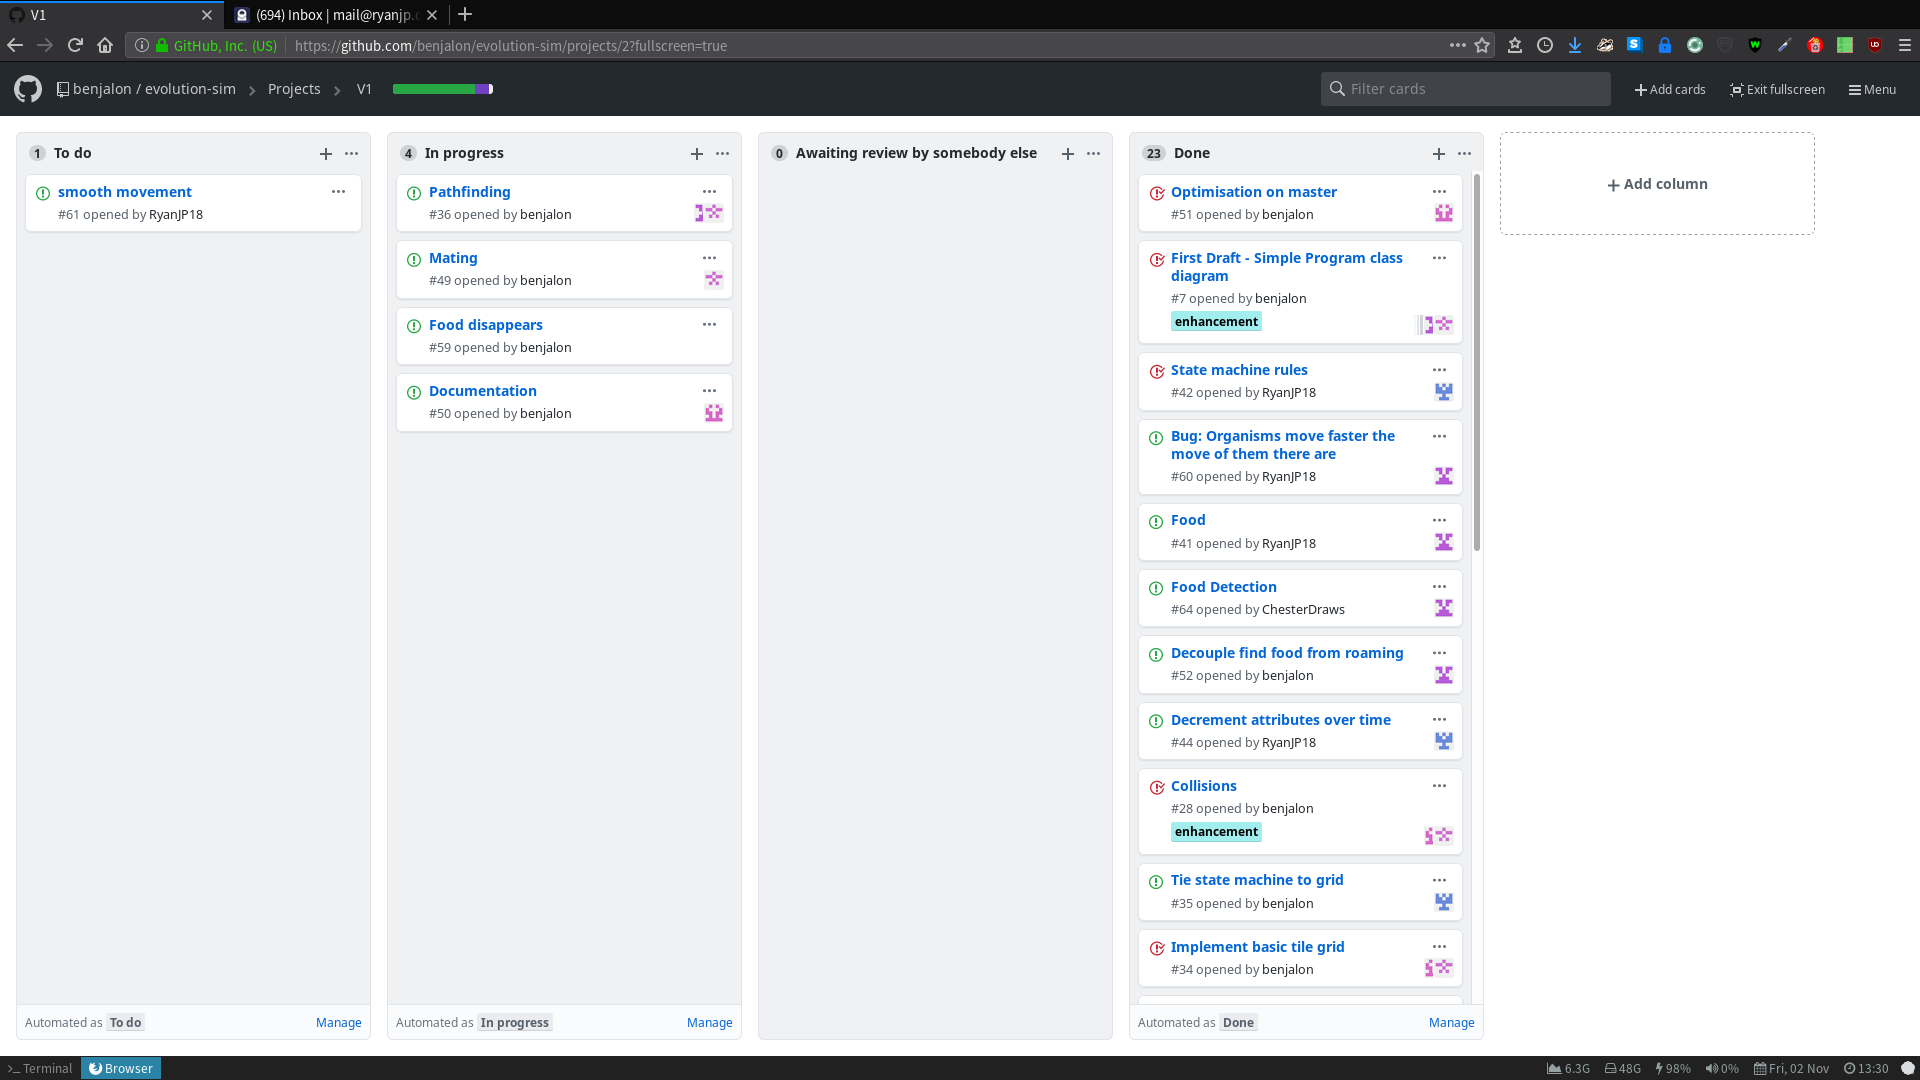
\includegraphics[width=1\textwidth]{gitproj}
\end{figure}

\begin{figure}[H]
	\caption{GitHub Issue Tracking}\label{gitissue}
	\centering
	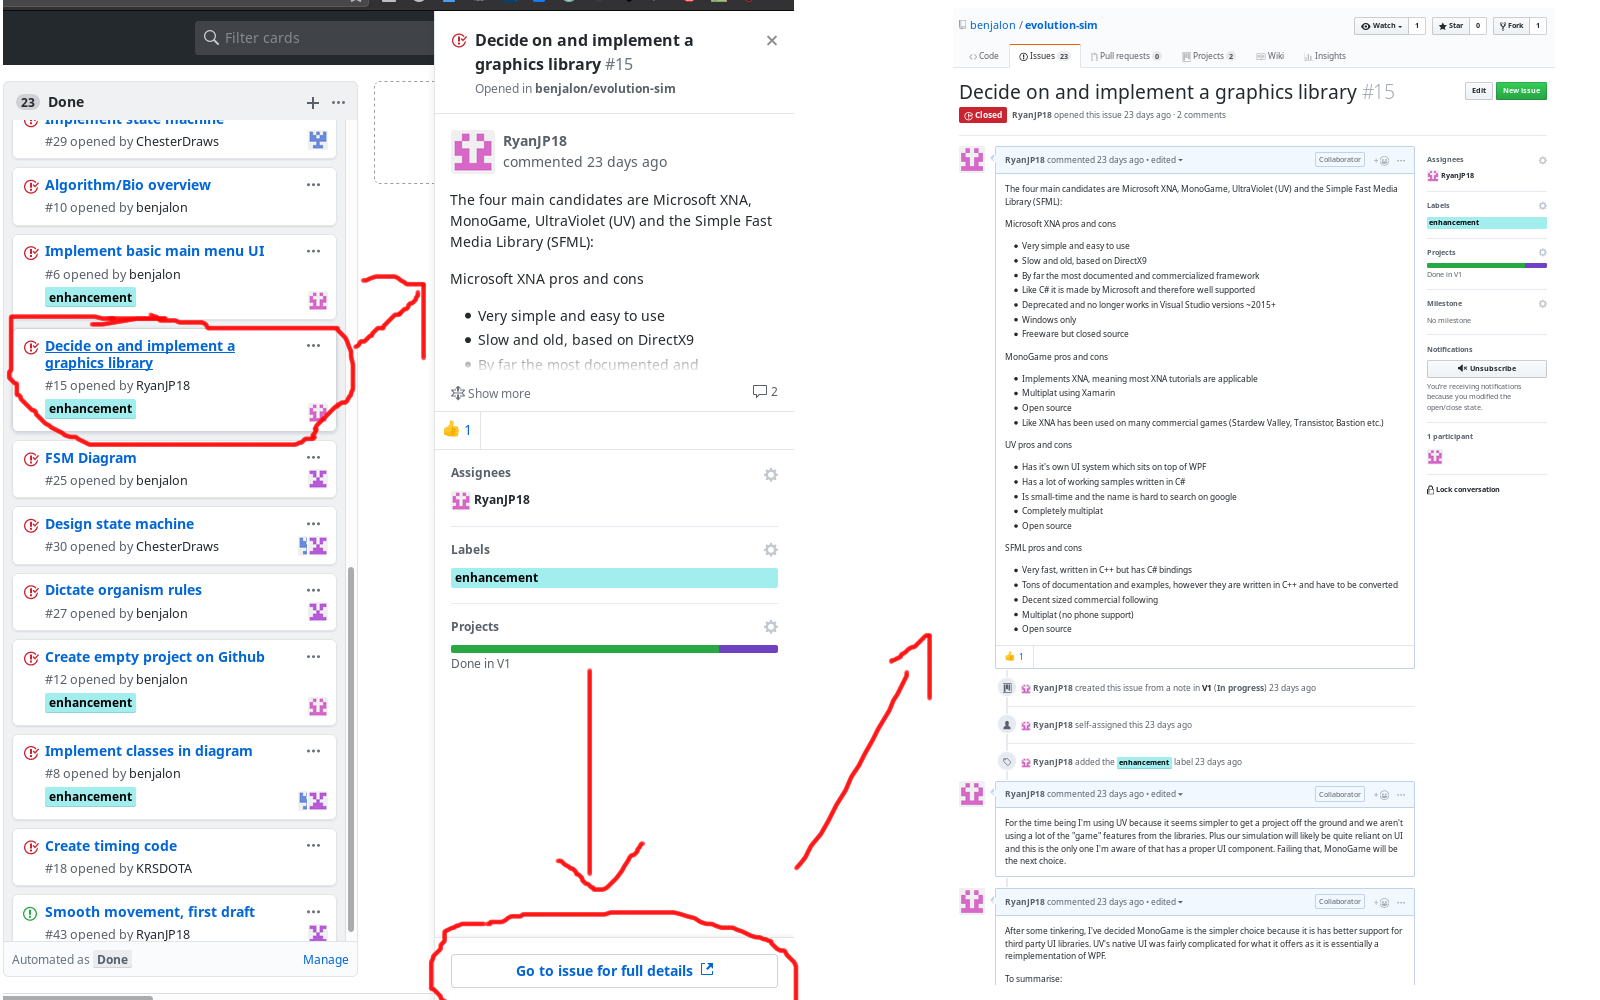
\includegraphics[width=1\textwidth]{gitissuetrack}
\end{figure}

Using Git, each ticket is developed on a unique feature branch. When code-complete, it is sent for pull request (i.e. peer review) before it can be merged into master. This system is enforced through a merge lock on master which only allows branch merges as opposed to direct commits. Additionally, these merges are rejected by the system unless it is reviewed by one other person. This system helps ensure the quality of master for branching at all times, avoiding situations where development is halted due to a buggy code-base. Additionally, these pull requests are able to function as a form of white-box testing as discussed in (Section~\ref{testing}).

Other project management tools used throughout the project include Microsoft OneNote for collaborative documentation and WhatsApp for quick discussion and meeting scheduling.

\section{Code Architecture}\label{architecture}
The SOLID principles define five guidelines which are used as the guiding principles in the project's architecture to ensure that code is maintainable and easy to understand \cite{kelmendi}:
\begin{itemize}
	\item Single Responsibility: Every class should have only one responsibility to prevent the class being susceptible to requirement changes.
	\item Open-Closed: Classes should be open to extension but abstraction should be used to avoid the need for rewrites on the extended code.
	\item Liskov Substitution: Derived and base classes should be substitutable.
	\item Interface Segregation: Keep interfaces simple to avoid bulk from implementing unnecessary properties.
	\item Dependency Inversion: Keep abstract code abstract by avoiding dependencies on low level code.
\end{itemize}

An example of how this has influenced design can be seen in the choice to split Grid from StateMachine. Although both handle moving and positioning organisms, Grid is treated as the ``graphical brain``, positioning organisms and drawing them at their positions, whereas the StateMachine is used as the ``logical brain``, dictating the behaviour which causes the organisms to be repositioned in the first place. This separation of concerns can also be seen in the namespaces, for example EvolutionSim.StateMachine, EvolutionSim.TileGrid, EvolutionSim.Data and EvolutionSim.UI.

Another example is through having GridItem function as a base class for Organism and Food. This swappable base is important due to the Tiles of Grid accepting either as a potential inhabitant. This swappable nature would not work if the Liskov Substitution principle was not applied.

To ensure a clean and consistent code-base, the official Microsoft C\# conventions are applied where possible. Notable examples include placing braces on a new line, using camelCase for variable names and avoiding one line if statements \cite{microsoft}.

\section{State Management}\label{statemanagement}
Within the simulation all organism behaviour is dictated by a finite state machine which contains a set of states and rules for moving between them. The StateMachine class is passed State objects which are essentially a lookup table for each state transition. Based on supplied information, the StateMachine determines which state the Organism should transition to and throws an exception if it determines the move to be illegal, for example it is impossible for an Organism to move directly from ``Mating`` to ``Eating`` through the Action ``FoundFood`` as the Organism must be in the ``Roaming`` state in order to reach this clause.

The StateMachine also contains two methods to drive organism behaviour: CheckState and DetermineBehaviour, which are both called every cycle of the Update loop. CheckState is responsible for checking that each Organism is in the correct state based on the rules defined for the simulation, for example if an organism is currently in the ``Roaming`` state, but it's hunger levels have dropped below 0.4, this would mean that the organism must now move into ``SeekingFood``. After the state is checked, DetermineBehaviour defines how the Organism should behave within this state.

\section{Crossover Algorithm}\label{crossover}
The initial crossover algorithm took an average from parent attributes and applied some random variations to these numbers. While effective and efficient in getting the general concept implemented, it was not complex enough to provide diversity in the simulation.

The improved crossover algorithm utilizes a probability class to generate a gaussian variable to provide implicit changes in the organisms and prevent stagnation. This is achieved by using a single component of the Box-Muller transform, a method traditionally used for gaussian estimation in a cartesian plane \cite{box1958note}, however in the case of our simulation we simply need to model the severity of each mutation. Once the gaussian variable has been calculated this is passed to a function which determines the severity of mutation based on the distance from the mean and which side of the distribution it falls on.

\section{Tile-Based Movement}\label{grid}
A common method of implementing movement in a simulation is by constraining it to a grid. This is useful because the number of movement states becomes finite and better lends itself to algorithms for path-finding. In terms of efficiency, a grid also reduces the need for collision detection between simulation elements by mediating on the movement between tiles. Linear interpolation is also applied to all tiles movements so that the organisms move smoothly rather than ``teleporting`` between them.

Within code, the Grid class holds a collection of Tiles within a jagged array which can each potentially hold a GridItem inhabitant. Within this collection, each index maps the tile to a screen position using the equation:
\[tilePos = offset + (tileIndex * TILE_SIZE)\]

\section{Pathfinding Algorithm}\label{pathfinding}
Pathfinding is a key component in the simulation and several implementations were considered. In terms of simplicity, DFS produces fast results but is naive and requires a large amount of time and memory to find the shortest route. Dijkstra's algorithm is an improvement because it applies a difficulty based on the movement cost to a destination, but is expensive as it compares equally and needlessly expands difficult locations without considering direction. Finally, at least for single-point to single-point searches (as used in this project), A* is considered the fastest algorithm \cite{belwariar} due to its improvement upon Dijkstra's with a heuristic. 
\[A* Algorithm: f(n) = g(n) + h(n)\]
In the above formula g(n) refers to the difficulty of a tile, used to handle different terrain types such. The h(n) is the diagonal distance between the two points and f(n) refers to the sum of g(n) and h(n).

A* is implemented in code by creating a Node object for each Tile, each holding a reference to the previous Node, its Grid position, the destination's distance and the difficulty in reaching it. To calculate the g(n) difficulty value, the terrain type of the Tile is taken into account and for the h(n) distance value, the diagonal distance between the two points is calculated by taking the maximum value of either the goal Tile's x coordinate minus the current Tile's x coordinate or the same for y coordinates. Nodes to be evaluated are stored in open and closed collections which are manipulated until a path to the goal is found.

\section{Optimisation}\label{optim}
Optimisation is important for the project due to its requirement in handling a large number of organisms without noticeable lag. By default, MonoGame's render loop updates and draws at sixty frames per second. Should the update logic fail to complete within this ~16-17ms time-frame then it delays the draw call, which lowers the simulation's frame-rate. This has further knock-on effects where the draw calls become progressively more delayed and eventually cause input lag on the UI. As the update method is essentially the primary path through the code, it calls into several loops to cycle through the items which make up the simulation. There can be several hundred objects to iterate through during any given Update loop and keeping this entire iteration within the acceptable ~16-17ms limit required a great deal of optimisation. Despite this, optimisation was a task left until it became a problem following the argument that ``premature optimization is the root of all evil`` \cite{knuth} by introducing bugs and making code less readable. 

As the simulation grew in size, loop optimisation became an issue particularly for state management and path finding. To improve this, variables are typically declared outside of loop scope to prevent them being redeclared on each iteration. Other standard optimisations such as caching the collection length ahead of time and avoiding high precision calculations are also applied. The grid's collection for storing tile objects is also a jagged array as opposed to a multi-directional one which is more efficient to loop over.

From an more architectural perspective, the grid system is also a form of optimisation. By constricting organism movements to a grid the simulation is able to cut down on the need for collision detection, which would otherwise have been a bottleneck for the system. This would have required exponentially more computation as organisms are added because each organism would need to check the itself against all others.

\section{Multi-threading} \label{multithreading}
The path-finding code was designed to run on a multi-threaded system to help stabilize overall system runtime, as well as naturally separating out tasks which can be asynchronously performed. It works by creating a pool of worker threads which can be delegated tasks to free up the main thread of execution, the ThreadPool class handles the queueing and waiting of threads as well as their destruction and creation. By pooling threads, stuttering through on-the-fly thread creation is avoided as much as possible.

\chapter{Implementation} \label{implementation}

\section{Object Oriented Analysis}\label{ooa}
An object oriented analysis was produced to gain an understanding of the problem domain and identify classes for the initial class diagram (Figure~\ref{ooa-breakdown}).

\section{UML}\label{uml}
Taking the potential classes identified in Section~\ref{ooa}, a class diagram was produced (Figure~\ref{classdiagram}) which was continually updated throughout the project but keeping its key themes. Figure~\ref{classdiagram-2} shows the final class diagram produced in this project which was used to identify the growing issue of coupling within the project. As discussed in Section~\ref{architecture}, the project was split into namespaces each housing components relating to their tasks. Communication between namespaces (except EvolutionSim.Utility and EvolutionSim.Data) is discouraged and the team was able to eliminate unnecessary imports through this diagram.

Furthermore, a requirement of the classes is that they aim to encapsulate their data and provide abstraction in information to make the code more manageable across the team. For example, code relating to a component such as the weather system is kept isolated within its class. The diagram also illustrates how this is achieved through inheritance, where base classes are generic and intricate functionality is extended further down the hierarchy. The main example of this can be seen in GridItems, essentially generic tile-based sprites, Food and Organism.

Due to the simulation's dependency on a complicated state management system, a state diagram was also created to identify how organisms would act (Figure~\ref{state-diagram}).
\section{Tools}\label{tools}
The simulation was identified to have a large dependency on computation due to the fact that there could be upwards of one hundred organisms on screen at any one time and each of them would require state management, path finding and collision detection. For this reason, C++ seemed to be the natural choice due to the speed benefit of dynamic memory management. However, upon further research it was found that C\# had a more diverse set of 2D graphics libraries with C++ libraries typically focused on 3D rendering.

A comparison was made between several popular 2D graphics libraries available in C\#, shown in Figure~\ref{library-comparison}, with MonoGame being chosen.

\section{Product Versions}\label{versioning}
In keeping with the spirit of iterative development, the projects aim to produce a new product at the end of each sprint. This ensures that at any given time, the active project board matches the current release version. Each version aimed to iterate upon the previous release with features taken from further down the MoSCoW analysis (Figure~\ref{version-table}).

\smallskip 
\begin{figure}[H]
	\caption{Product versions and sprints} \label{version-table}
	\centering
	\begin{tabular}{c|p{0.7\textwidth}|l}
		Version & Goal & Deadline \\ \hline
		0 & A proof of concept to test the chosen technologies & Tuesday week 2 \\ \hline
		1 & A fully functioning basic simulation with all of the ``Must Have`` components from the MoSCoW analysis & Friday week 6 \\ \hline
		2 & Improvements on V1 simulation and ``should have`` objectives: A* path-finding, improved crossover algorithm, carnivores and a better time system. & Friday week 8 \\ \hline
		3 & Path finding performance enhancements and bug fixes & Friday week 10 \\ \hline
		3 & More ``Should Have`` objectives and missing functionality. Primarily eating, dying, mating, terrain and a time system. & Friday week 12 \\ \hline
		4 & Final missing features: Weather system, carnivores and prey, particle effects. & Christmas \\ \hline
		5 & Loose ends, bug fixes and report updates. & Project deadline \\ \hline
	\end{tabular}
\end{figure}
\smallskip 

\section{Proof of Concept}
A proof of concept was made with the chosen technologies to avoid a situation where the UML modelling and code architecture was planned according to a language or tool which was a poor fit for the project. It aimed to simply draw a number of organisms to the screen using the chosen graphics framework which could be manipulated using a simple place-holder UI.

\begin{figure}[H]
	\caption{Proof of Concept}\label{poc}
	\centering
	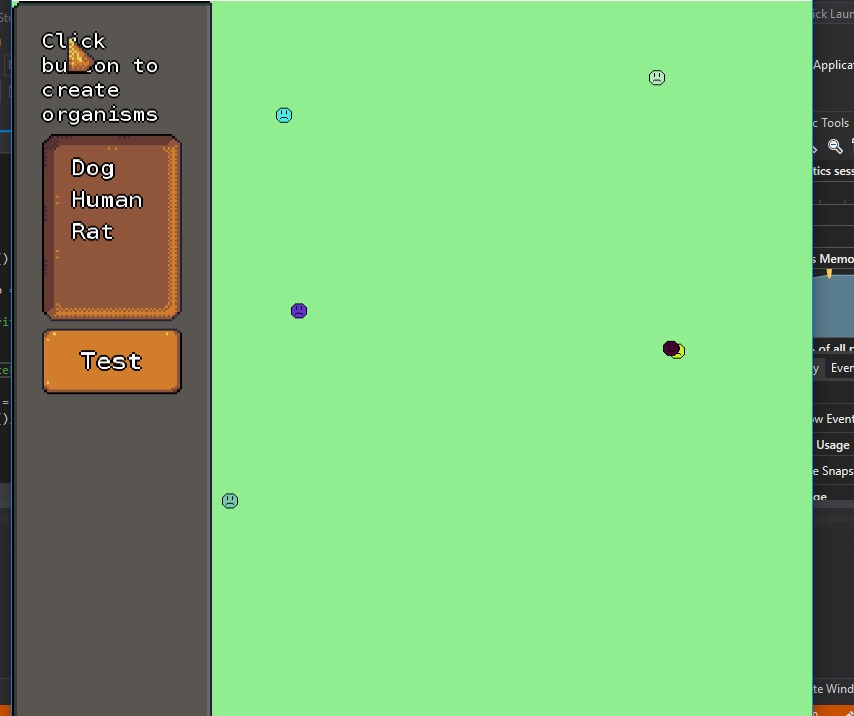
\includegraphics[width=0.8\textwidth]{poc}
\end{figure}

\section{Final Version}
The final version of the product was able to implement all ``Must Have`` and ``Should Have`` requirements in addition to several ``Could Have`` objectives. Compared to the proof of concept it also received a graphics overhaul and a much more sophisticated UI.

\begin{figure}[H]
	\caption{Final Version}\label{final-ver}
	\centering
	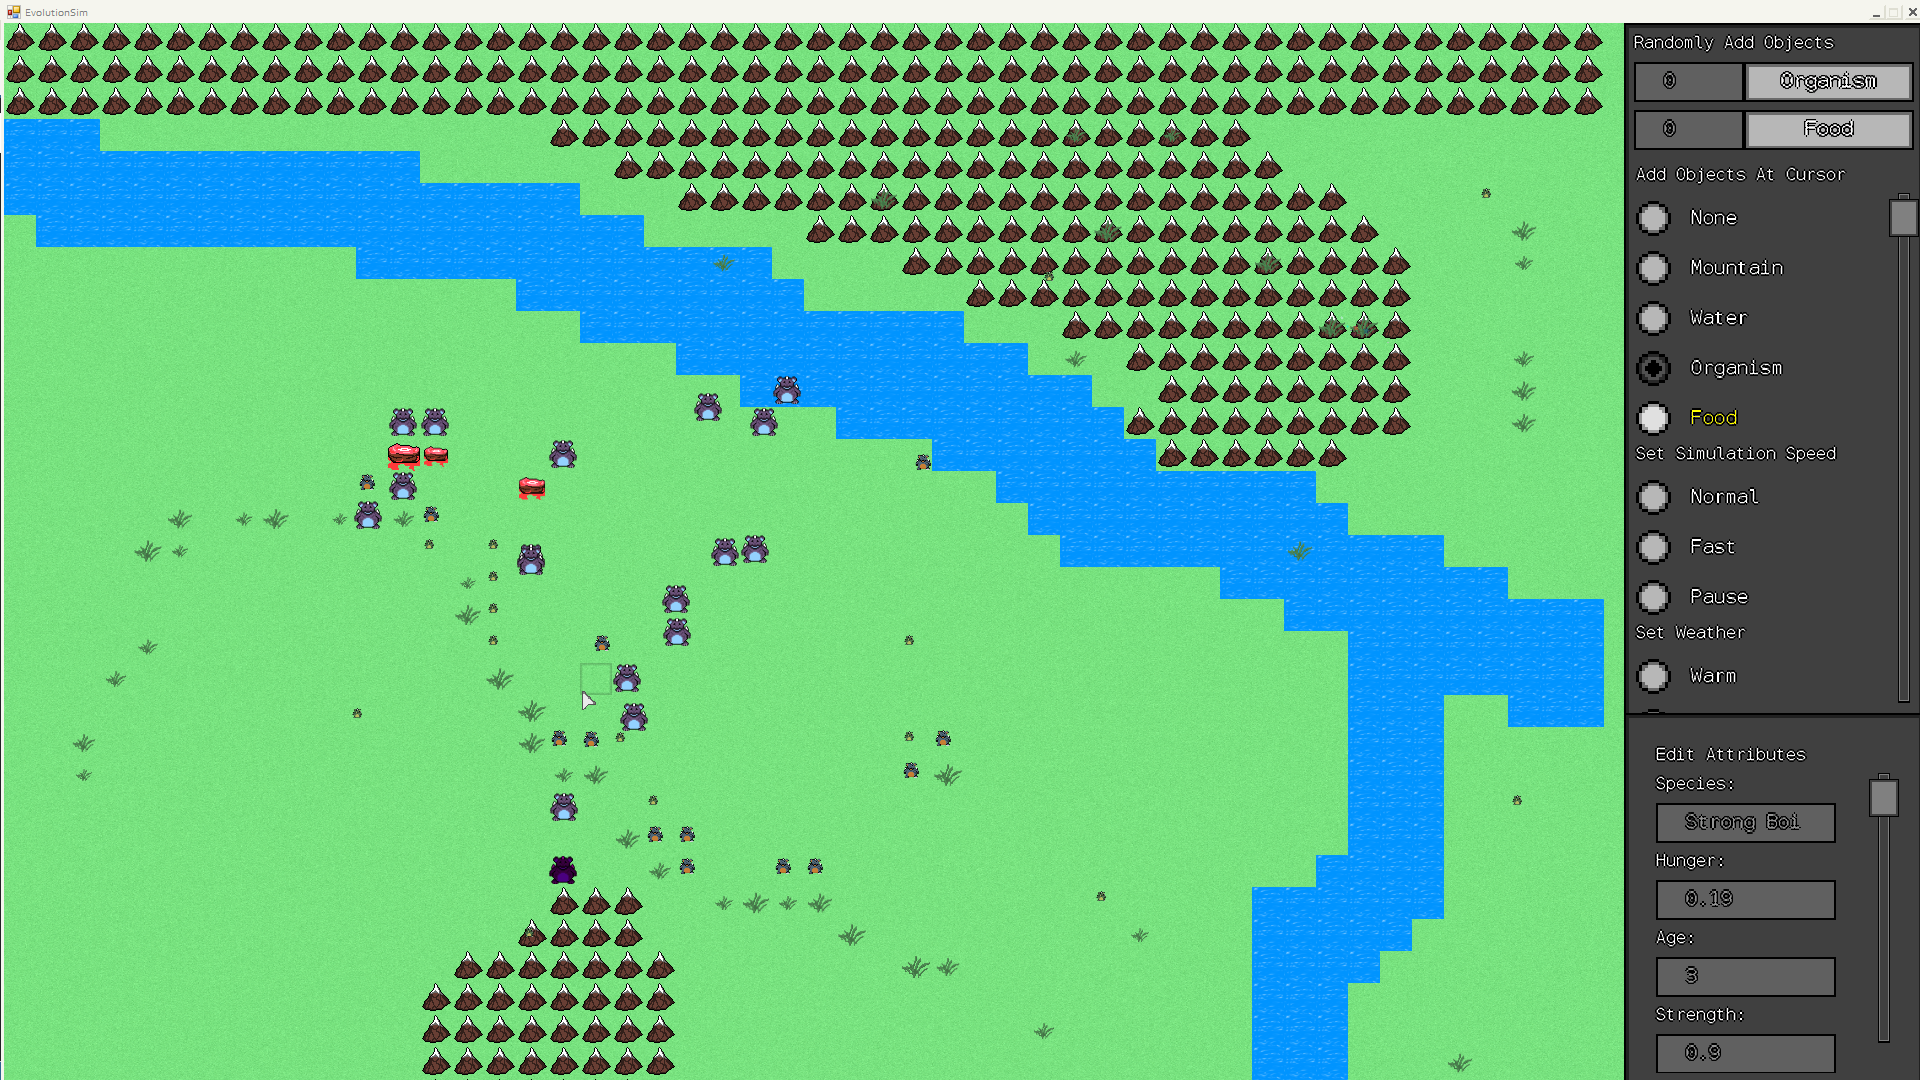
\includegraphics[width=0.8\textwidth]{final-ver}
\end{figure}

\chapter{Testing}\label{testing}
Throughout the project dynamic white box testing was carried out in the form of pull requests and code reviews using GitHub. Agile development encourages testing to occur at all stages of the project, rather than as a formalised testing phase at the end. For this reason, to assure the quality of the software throughout, strict rules were enforced on GitHub by locking commits to the master branch. All code was required to be tested by and reviews by a member of the team other than the one submitting the code. In this code reviews, issues such as failure to keep to the coding standards, poor architectural decisions or bugs were highlighted and requested to be fixed before the merge was approved.

Dynamic black box testing was used extensively throughout the project. It was also dedicated a sprint to itself at the end of the project (Figure~\ref{gitbugfixing}).

\begin{figure}[H]
	\caption{Final Bugfixing Sprint}\label{gitbugfixing}
	\centering
	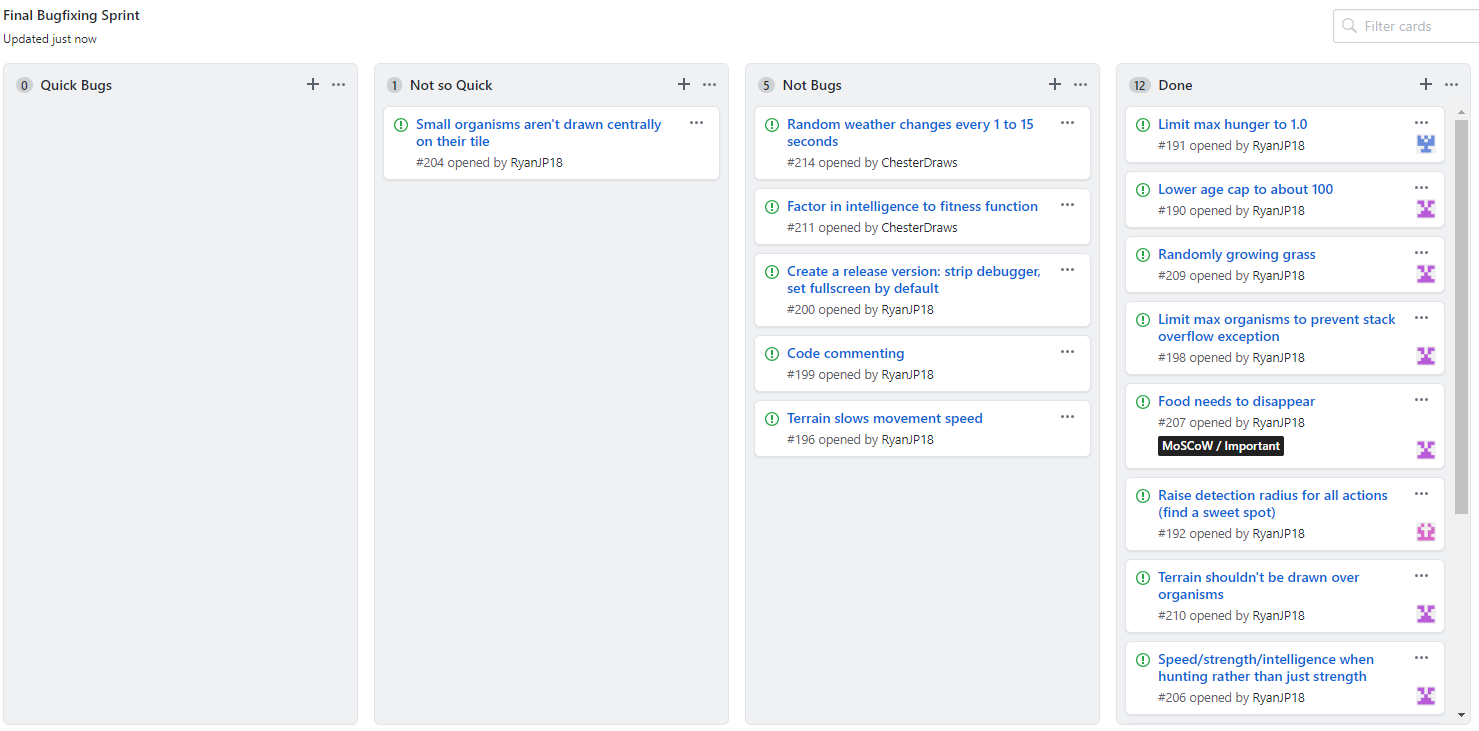
\includegraphics[width=0.8\textwidth]{gitbugfixing}
\end{figure}

\section{Requirements Testing}
Dynamic black box testing was also performed on the simulation to ensure that the initial project requirements were met. This was achieved through ``test to pass`` and ``test to fail`` approaches to maximise the bug and issue reporting. This test plan can be seen in Figure~\ref{requirements-testing}.

In order to prove equilibrium, the simulation was left running for an hour while logging the population count over time (Figure~\ref{equilibrium-test}). Though the population fluctuates, it always returns to equilibrium given time.
	
\begin{figure}[H]
	\caption{Equilibrium Test}\label{equilibrium-test}
	\centering
	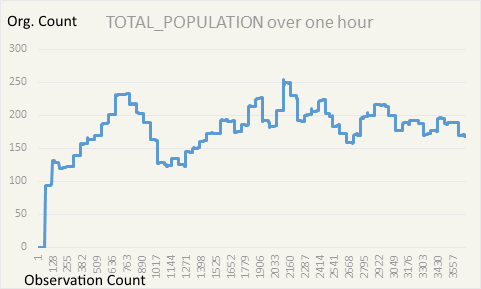
\includegraphics[width=0.8\textwidth]{equilibrium-test}
\end{figure}
	
\section{Code Metrics}
Visual Studio provides tools to analyse a project, providing insight into the maintainability, coupling and cyclomatic complexity of a project. The overview of these results can be seen in Figure~\ref{metrics-1} and the specifics in Figures \ref{metrics-2} and \ref{metrics-3}.

\begin{figure}[H]
	\caption{Code Metrics Namespaces}\label{metrics-1}
	\centering
	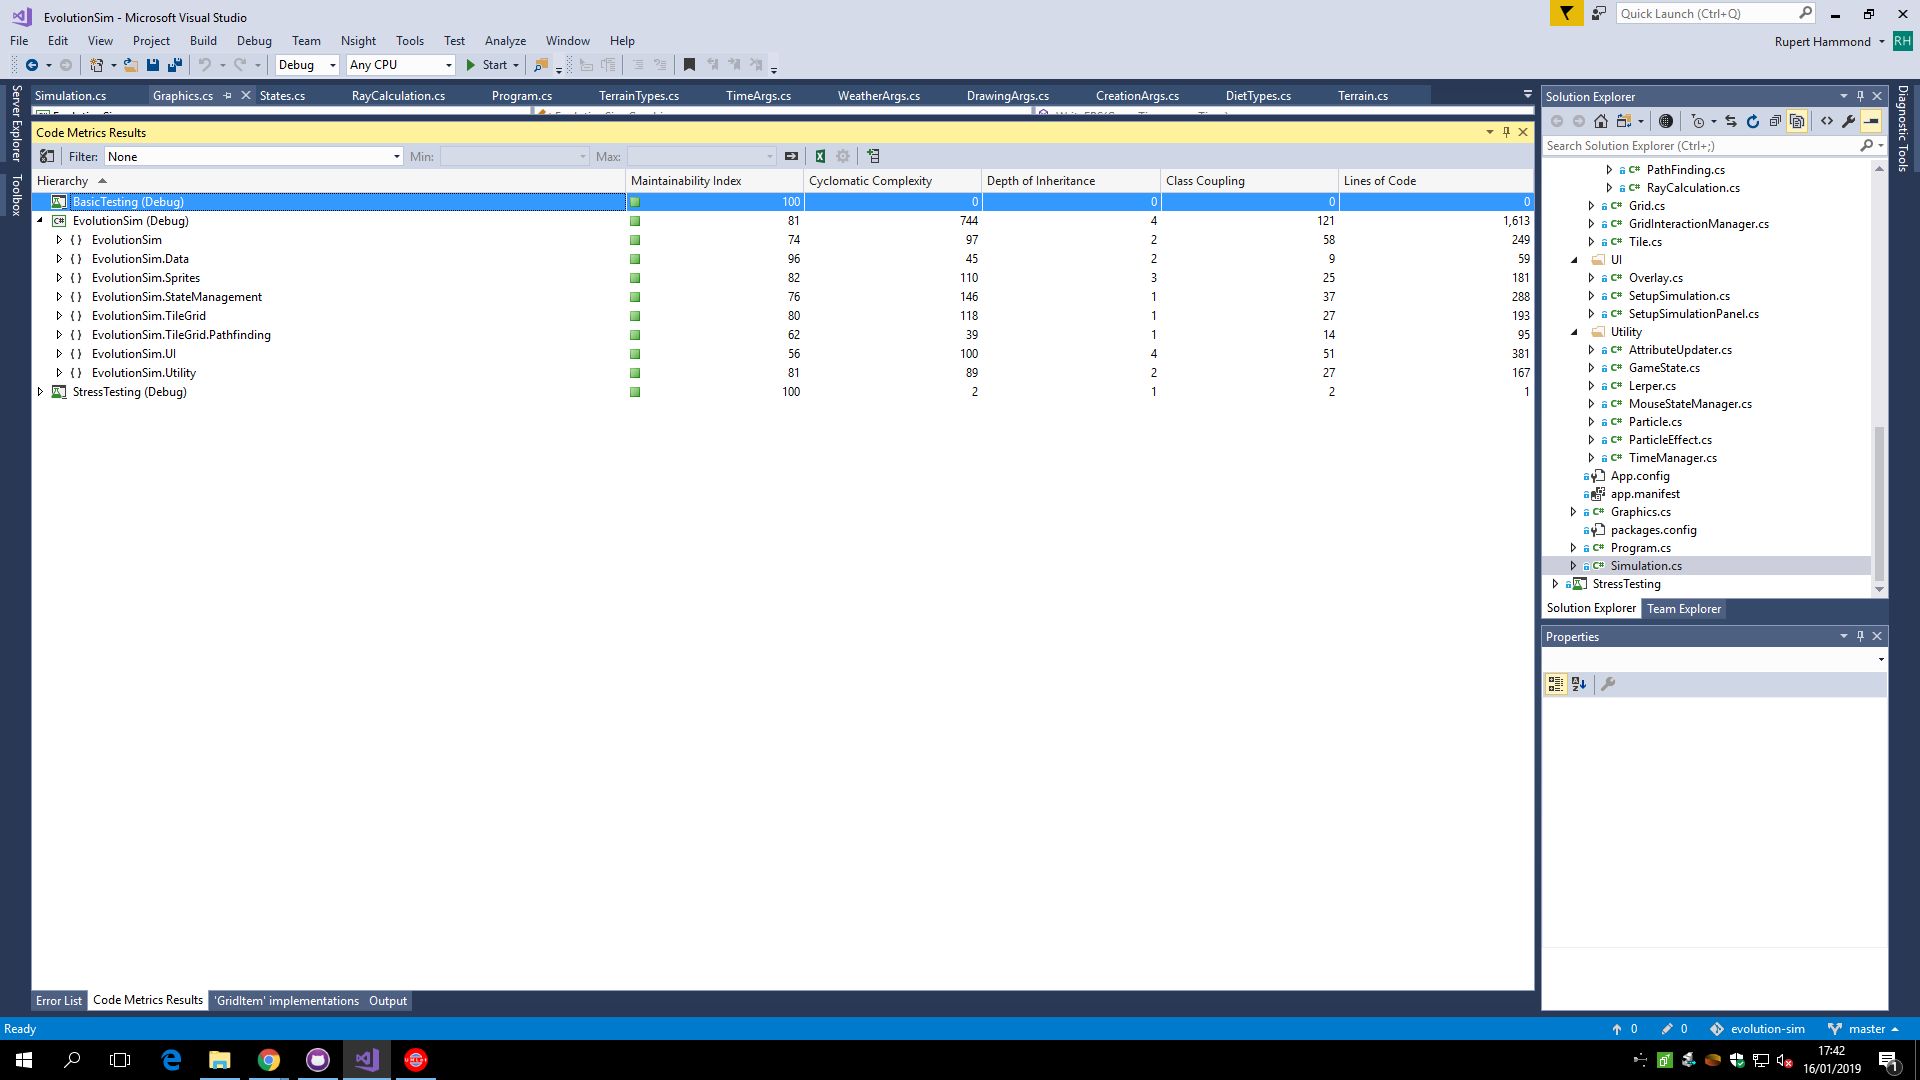
\includegraphics[width=0.8\textwidth]{metrics-1}
\end{figure}

\begin{figure}[H]
\caption{Code Metrics Classes Pt. 1}\label{metrics-2}
\centering
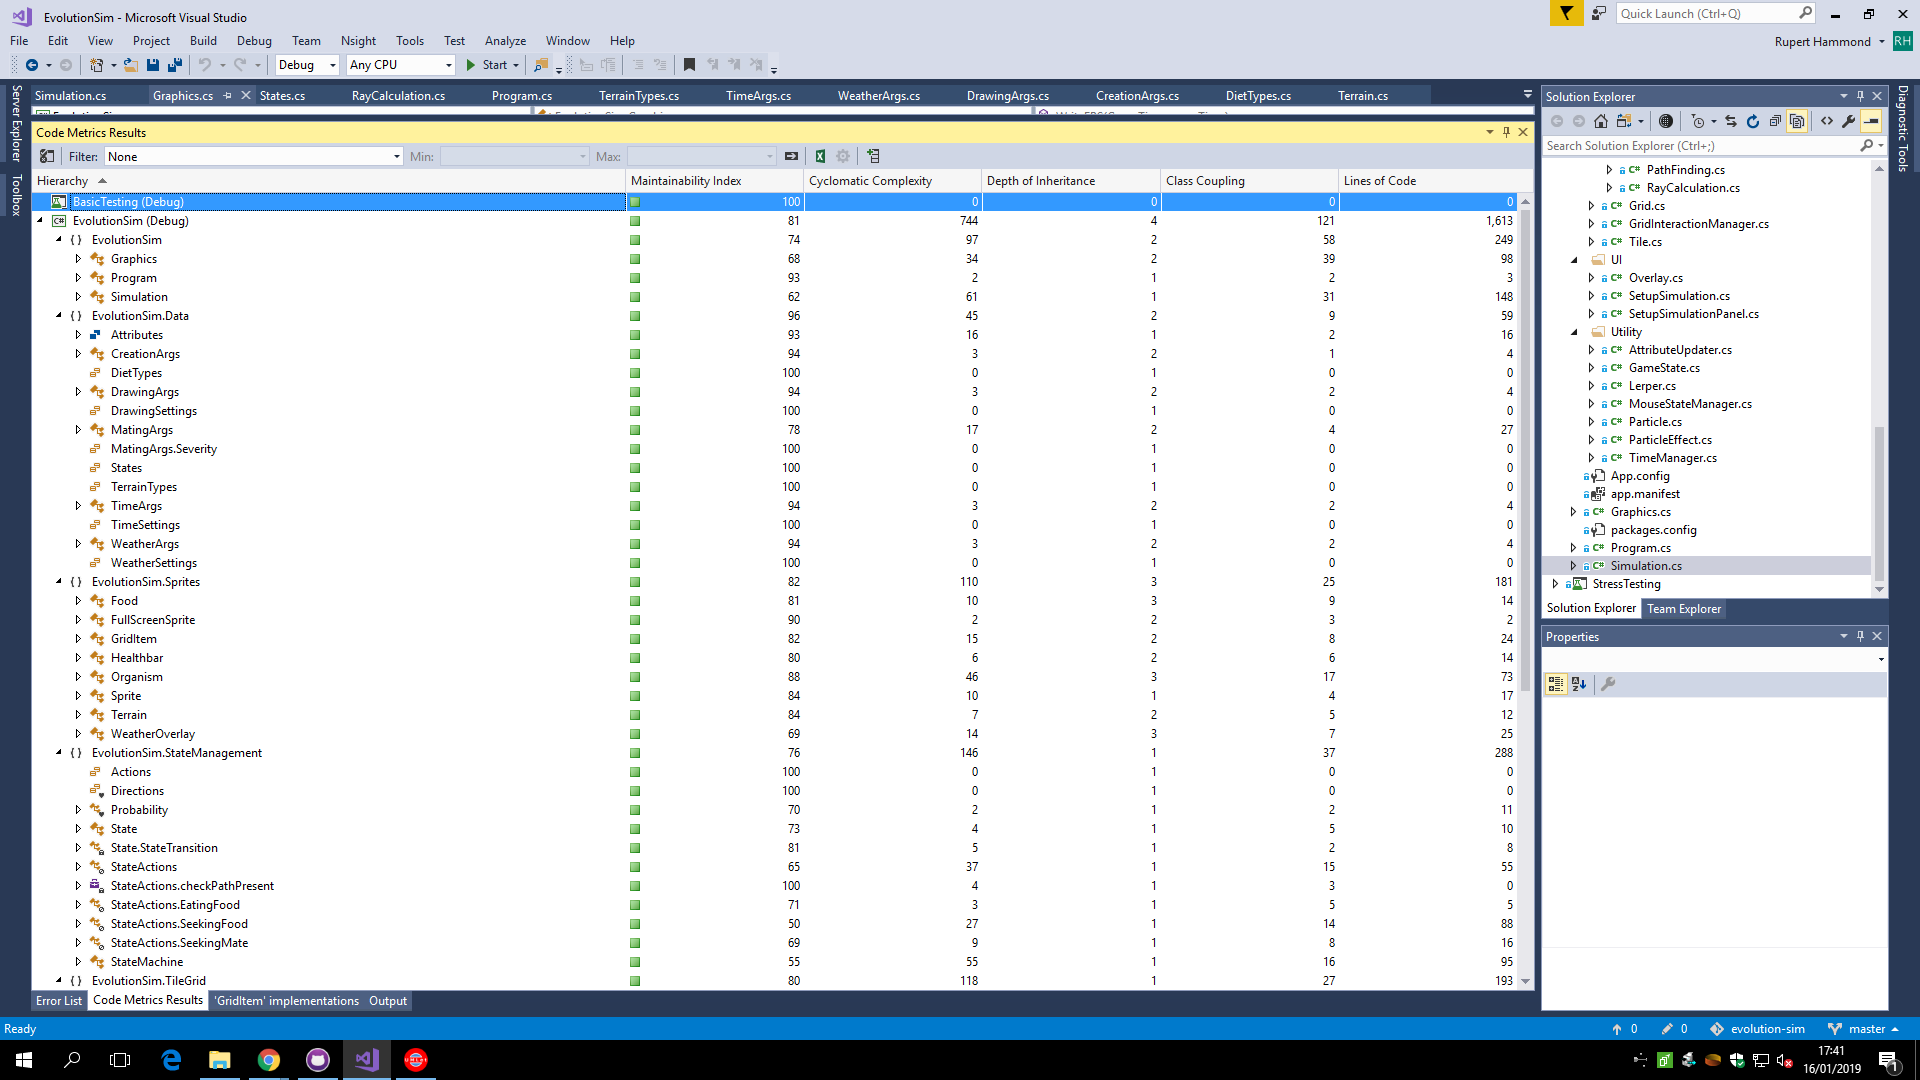
\includegraphics[width=0.8\textwidth]{metrics-2}
\end{figure}

\begin{figure}[H]
	\caption{Code Metrics Classes Pt. 2}\label{metrics-3}
	\centering
	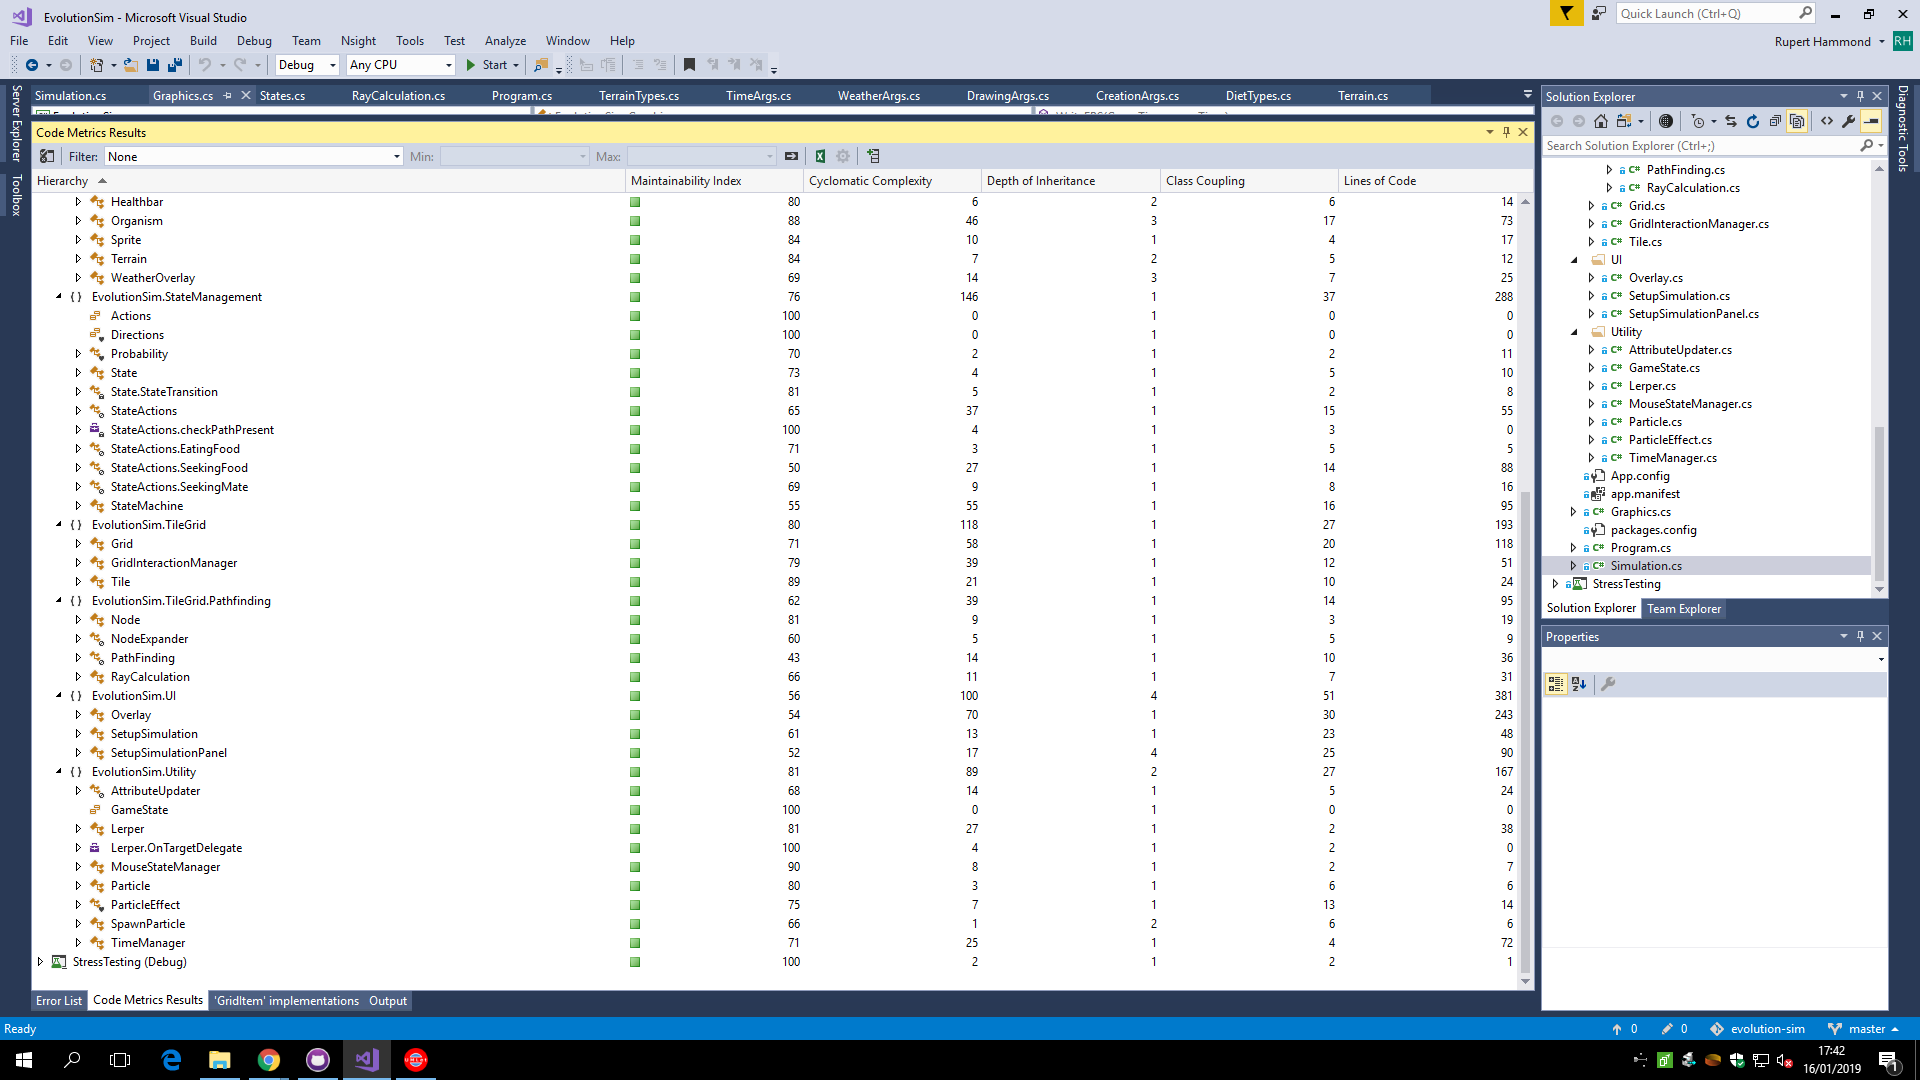
\includegraphics[width=0.8\textwidth]{metrics-3}
\end{figure}

The maintainability rating estimates how difficult code is to maintain by testing how long and heavily interlinked it is. The project has an overall maintainability score of 81 out of 100, which ranks green (the highest rating). Individual classes within the project report scores between 56 and 96 and this difference can typically be explained through how algorithmic or state-based a class is. In general, any score above 50 is considered good in the Visual Studio maintainability metric.

Complexity measures the number of decisions present within a block of code plus 1. This generally correlates to how easy the code is to comprehend and therefore how easy it is to fix or add to. The worst score in the project can be credited to the EvolutionSim.StateMachine namespace, which is natural. The state machine handles all of the branching for organism behaviour and is essentially the logical brain of the project. Overall, it would be desirable for the project to aim to lower these scores moving forwards as cyclomatic complexity causes many problems both in terms of maintainability and robustness.

Finally, coupling is measured as a value of how many other classes or imports a class is dependent on. This was deemed the most important factor to reduce throughout the project and much effort was placed on reducing coupling where possible, particularly between namespaces. The worst offenders for coupling, either by design or otherwise, are StateMachine, Organism and Grid. 

\chapter{Discussion}\label{discussion}
At all points in the project, one of the systems that worked well was the iterative approach to development. Categorising tasks into sprints, where high priority tasks were tackled earlier in the project and luxury additions were dealt with later ensured that the product development kept moving forward, ensuring a high level of motivation. Additionally, the team was able to re-evaluate the importance of aspects of the simulation continuously, allowing it to grow from the initial plans. The success of this iterative development is due to the effectiveness of the project management and the tools chosen to support it.

However, although the project management as a whole was effective, there were several areas that it could be improved upon in future projects. Beginning the project with a proof of concept was a great decision in the short term, but the benefits it brought were diminished somewhat by a poor choice of following tasks. Tackling tasks in order of priority produced mixed results because certain core functionality such as a sophisticated roam function and a time manager were left until far too late in the project. This meant that when they were eventually implemented, other features had to be retroactively fitted to handle them, which led to some redundancy and therefore wasted time.

A key strength of the simulation lies in its ability to handle a large amount of computation with minimal lag. As discussed in Section~\ref{optim}, within the code there are many advanced algorithms such as the A* path-finding which must apply to a great number of objects and finish computing within a tight schedule. Through careful consideration to optimisation, frequent rewrites of inefficient areas of the code and a system of running complex algorithms on separate threads, the simulation is able to handle upwards of a thousand elements without noticeable issue.

In terms of functioning as an evolutionary sandbox, the simulation has reached a level of intricacy whereby the organisms will evolve differently depending on the simulation parameters. In a map which is segregated into parts by the presence of terrain, camps of organisms will evolve with differing attributes depending on what has become important to their survival. For example, an area which has seen a rare mutation in strength will have larger organisms over time than a camp which did not acquire this mutation. Furthermore, whether herbivores, omnivores or carnivores become the majority varies significantly across multiple simulations.

Likely the biggest shortcoming of the project is in its lack of variation of species. The team originally planned to have bird and fish species to add further meaning to the terrain system. A bird species for example would not receive a movement penalty when passing over water or mountains, a fish would also be impeded by water but would find all other ground impassable. The A* algorithm and simulation state management currently have the functionality to handle this kind of behaviour but due to time constraints, producing artwork and maintaining equilibrium with these new species was deemed not possible.

\chapter{Conclusion and Future Work}\label{conclusion}
Overall this project was ambitious in its aims to produce an evolution sandbox with some degree of interactivity and in many ways would benefit from more time. Despite this, many of the requirements (\ref{requirements}) and MoSCoW goals {(\ref{moscow}) allude to the attainment of an equilibrium within the ecosystem and this is something that has been tested to work in Section~\ref{requirements-testing}. In terms of the MoSCoW analysis, all core functionality identified in ``Must Have`` and ``Should Have`` have been implemented, while some attempt was made at implementing a program flow and particle effects from the ``Could Have`` objectives. For these reasons, the project could be argued to be successful.

If this project were to continue, the priority would be on implementing an improved hunting system. Due to time constraints, a system which had been developed using ray calculations and a new set of states had to be removed during the final stretch due to the presence of bugs. The system which replaced it is functional, but simplistic and not as elegant of a solution. With this feature in place, adding new species with more diverse attributes such as binocular and monocular vision and expanding the movement speed system to account for terrain differences and the speed attribute would follow this.

Finally, if this project were to be repeated again, one change would be to focus on having fewer but more sophisticated systems. Initial plans for this project were too ambitious and were not corrected until the mid-point, this led to redundancy in how time was spent developing the luxury systems.

\bibliographystyle{unsrt}
\bibliography{references}

\chapter*{Contributions}
The team has agreed on a 25\% contibution each as of the time of writing. Many tasks such as the proof of concept, research and planning were completed as a team .
\smallskip 
\begin{center}
	\begin{tabular}{c|p{0.4\textwidth}|p{0.4\textwidth}}
		Member & Ownership of/Major Contributions & Assisted on/Minor Contributions \\ \hline
		Benjamin Longhurst & \begin{itemize}
			\itemsep0em
			\item Project management [\ref{projectmanagement}]
			\item A* Pathfinding [\ref{pathfinding}]
			\item Testing [\ref{testing}]
			\item Report writing
			\item Spiral seek algorithm
		\end{itemize} & \begin{itemize}
			\itemsep0em
			\item Grid/tile system [\ref{grid}]
			\item Tile movement logic
			\item Bio. algorithms research [\ref{crossover}]
			\item Background research [\ref{background}]
			\item Organism attributes
		\end{itemize} \\ \hline
		Rupert Hammond & \begin{itemize}
			\itemsep0em
			\item State management [\ref{statemanagement}]
			\item State machine rules
			\item Organism attributes
			\item Hunting system
			\item Multi-threading [\ref{multithreading}]
			\item Mating system
			\item Crossover algorithm [\ref{crossover}]
			\item Unused ray calculations
			\item Spiral seek algorithm
		\end{itemize} & \begin{itemize}
			\itemsep0em
			\item Bug fixing
			\item Report writing
			\item Cooldown system
			\item Background research [\ref{background}]
			\item State UML [\ref{uml}]
		\end{itemize} \\ \hline
		Ryan Phelan & \begin{itemize}
			\itemsep0em
			\item Graphics setup [\ref{tools}]
			\item Grid/tile system [\ref{grid}]
			\item Report writing
			\item In-game UI
			\item Real-time attribute editing
			\item Drawing and selection system
			\item Particle effects
			\item Birth, death and eating events
			\item Spritework
			\item Terrain system
			\item Weather system
			\item Timing and cooldown system
		\end{itemize} & \begin{itemize}
			\itemsep0em
			\item Project management [\ref{projectmanagement}]
			\item Code architecture [\ref{architecture}]
			\item Code optimisation [\ref{optim}]
			\item HP bars
			\item Naive crossover [\ref{crossover}]
			\item Class UML [\ref{uml}]
		\end{itemize} \\ \hline
		Travis Payne & \begin{itemize}
			\itemsep0em
			\item Food system
			\item Advanced movement logic
			\item Simulation flow [\ref{statemanagement}]
			\item Multi-threading [\ref{multithreading}]
			\item Simulation set-up UI
			\item Bug fixing
			\item Miscellaneous tweaks
		\end{itemize} & \begin{itemize}
			\itemsep0em
			\item Code architecture [\ref{architecture}]
			\item Organism attributes
			\item Hunting system
			\item In-game UI
			\item Real-time attribute editing
			\item Naive seek algorithm
		\end{itemize} \\
	\end{tabular}
\end{center}

\chapter*{Appendix A}

\begin{figure}[H]
	\caption{MoSCoW Analysis}\label{moscow}
	\centering
	\begin{tabular}{c|p{0.8\textwidth}}
		Must Have & \begin{itemize}
			\itemsep0em
			\item Organism life cycle
			\item Genetic crossover algorithm
			\item Unique organism attributes such as health, age, strength, speed and resistances
			\item Organisms state determined by their unique attributes
			\item Unique organism attributes should be editable on the fly
			\item Simple UI Overlay
			\item Live edit of organisms
			\item Simple 2D graphics
			\item Herbivores and natural food sources
		\end{itemize} \\ \hline
		Should Have & \begin{itemize}
			\itemsep0em
			\item Weather/disease system
			\item Advanced path-finding algorithm
			\item Carnivores and predator/prey organisms
			\item Terrain variation, e.g. grass, mountainous, water
			\item Ability to pause, speed up and slow down simulation
		\end{itemize} \\ \hline
		Could Have & \begin{itemize}
			\itemsep0em
			\item Natural disasters
			\item Speciation (new species forming from heavily mutated organisms over time)
			\item A game log with charts and text output
			\item Spritesheet animation
			\item Particle effects, e.g. weather effects, running water, blood
			\item Program flow (start screen, simulation setup, end screen etc.)
		\end{itemize} \\ \hline
		Won't Have & \begin{itemize}
			\itemsep0em
			\item 3D graphics
			\item Scale realism
		\end{itemize} \\
	\end{tabular}
\end{figure}

\begin{figure}[H]
	\caption{Object Oriented Analysis Breakdown}\label{ooa-breakdown}
	
	\textbf{Specification} \\
	Objective: To make a simulation of evolution that reaches a stable point at some point.
	What does stable ecology mean? 
	\begin{itemize}
		\item Net number of organisms does not significantly increase or decrease over a given period of time.
	\end{itemize}
	\textbf{Requirements} \\
	Graphical representation of an organism.
	An organism has attributes such as:
	\begin{itemize}
		\item Health 
		\item Hunger 
		\item Speed
	\end{itemize}
	The organisms need to eat food which can either be other organisms or vegetation. 
	The organisms should breed and their attributes (representing genetics) will be crossed over to make a composite organism with random features within limit. 
	Environmental factors play a part in the life cycle and cold or hot climate can kill some organisms unless they have the specific resistances to temperatures. 
	Water should be present on the map which organisms can walk into but slows them down. Same with different terrain such as mountains. 
	
	\textbf{Real World Domain Environment:}
	\begin{itemize}
		\item Mountains
		\item Water
		\item Land
		\item Hot
		\item Cold
	\end{itemize}
	
	\textbf{Sprites and Organisms:}
	\begin{itemize}
		\item Herbivore 
		\item Carnivore 
		\item Plant
	\end{itemize}
	
	\textbf{Simulation:}
	\begin{itemize}
		\item State machine / brain
	\end{itemize}
\end{figure}

\begin{figure}[H]
	\caption{UML Class Diagram}\label{classdiagram}
	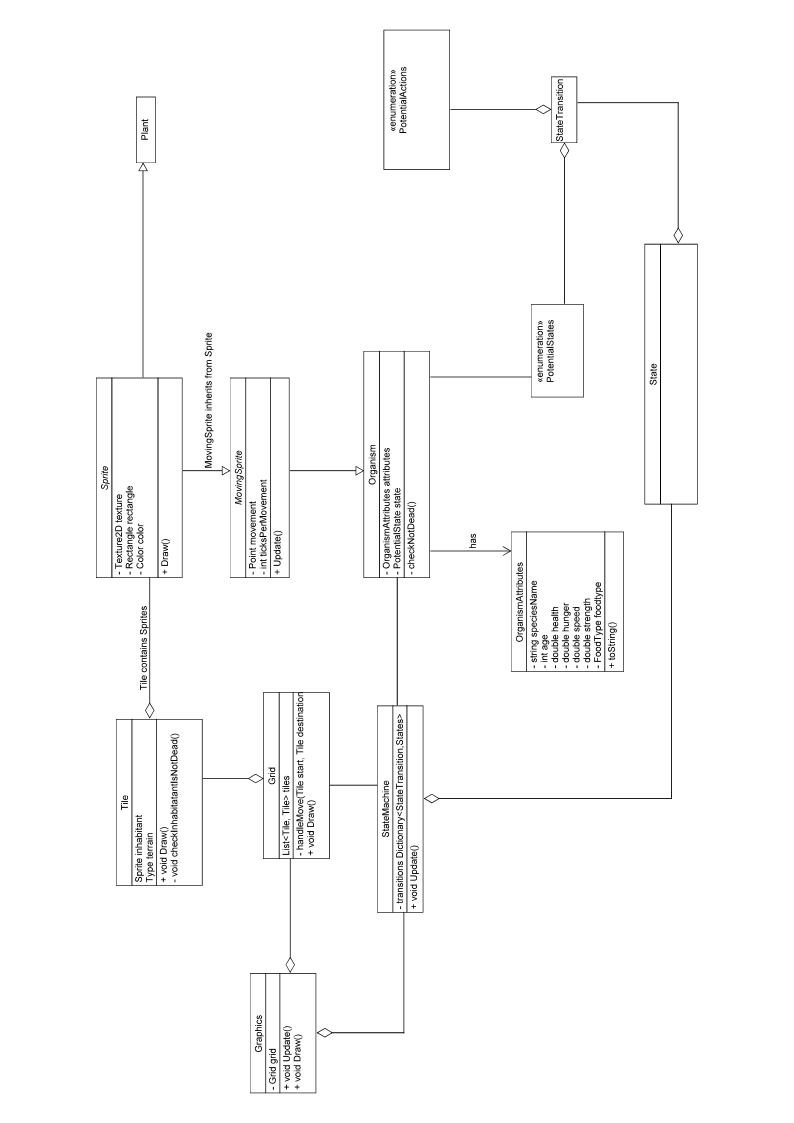
\includegraphics[width=\textwidth]{class-diagram}
\end{figure}

\begin{landscape}
	\begin{figure}[H]
		\caption{UML Class Diagram December}\label{classdiagram-2}
		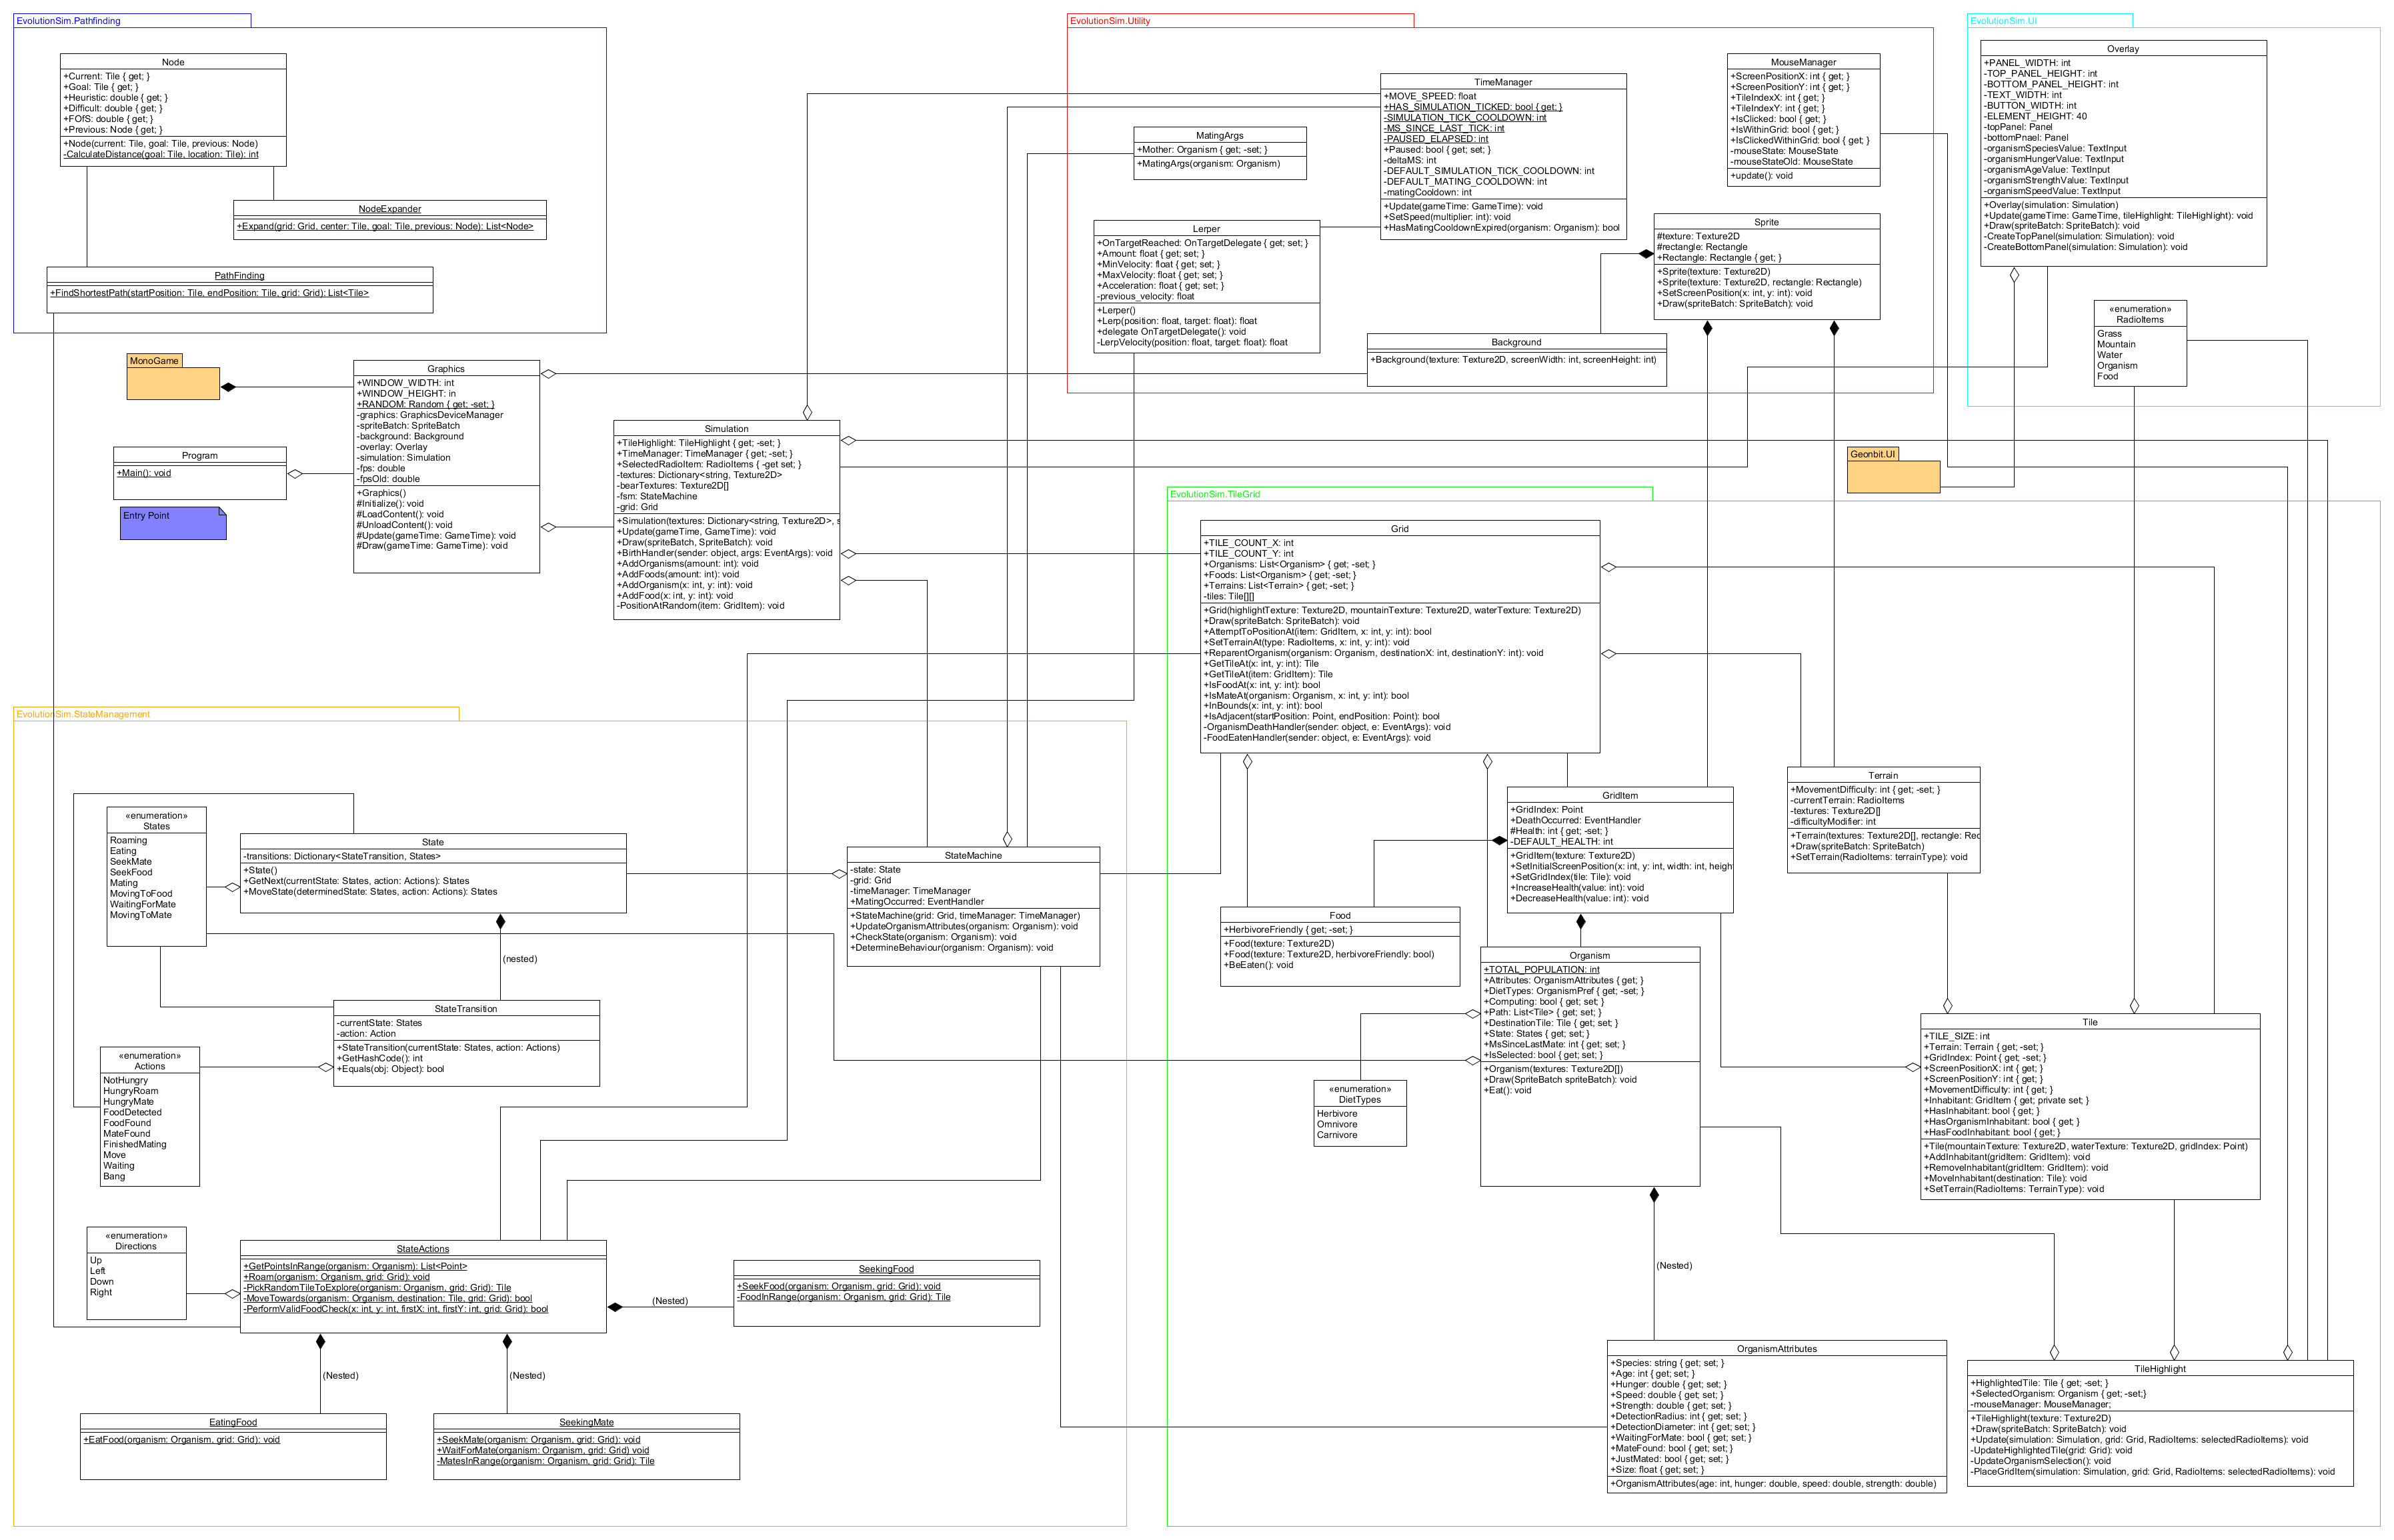
\includegraphics[height=\textheight]{class-diagram-2}
	\end{figure}
\end{landscape}

\begin{figure}[H]
	\caption{UML State Diagram}\label{state-diagram}
	\centering
	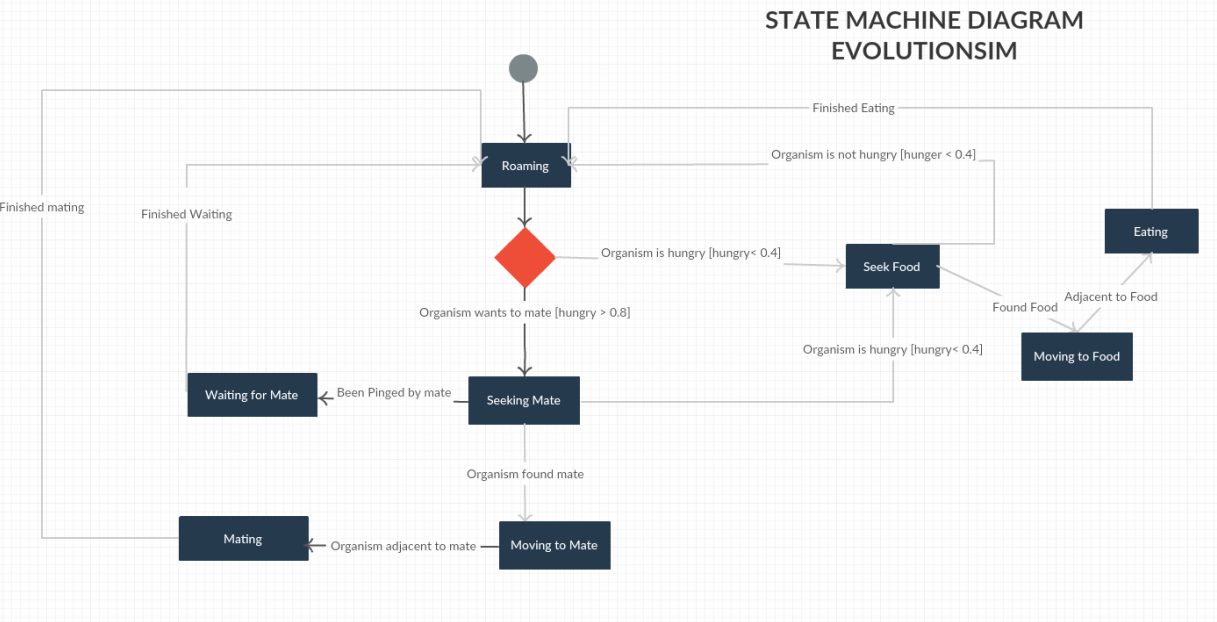
\includegraphics[width=1\textwidth]{state-diagram}
\end{figure}

\begin{figure}[H]
	\caption{Graphics Library Comparison}\label{library-comparison}
	\centering
	\begin{center}
		\begin{tabular}{c|p{0.4\textwidth}|p{0.4\textwidth}}
			Library & Pros & Cons \\ \hline
			Microsoft XNA & \begin{itemize}
				\itemsep0em
				\item Simple and easy to use
				\item Very well documented
				\item Well-used commercially
				\item Supported by Microsoft who also made C\#
			\end{itemize} & \begin{itemize}
				\itemsep0em
				\item Slow and old, based on DirectX9
				\item Deprecated and no longer works in Visual Studio 2015+
				\item Windows only
				\item Closed source
			\end{itemize} \\ \hline
			MonoGame & \begin{itemize}
				\itemsep0em
				\item Based on XNA with the same syntax, all of the XNA documentation is applicable
				\item Multi-platform but requires Xamarin
				\item Open source
				\item Has seen use on commercial games (Stardew Valley, Transistor, Bastion etc.)
			\end{itemize} & \begin{itemize}
				\itemsep0em
				\item Convoluted asset management system
			\end{itemize} \\ \hline
			UV & \begin{itemize}
				\itemsep0em
				\item Has a built in UI framework based on Windows Presentation Foundation (WPF)
				\item Truly multi-platform
				\item Open source
			\end{itemize} & \begin{itemize}
				\itemsep0em
				\item Convoluted asset management system
				\item Limited documentation, small time
				\item Little to no commercial use
			\end{itemize} \\ \hline
			SFML & \begin{itemize}
				\itemsep0em
				\item Very fast, written in C++ but has C\# bindings
				\item Well documented
				\item Some commercial use
				\item Multi-platform but no phone support
				\item Open source
			\end{itemize} & \begin{itemize}
				\itemsep0em
				\item C\# bindings are slightly behind on updates
				\item Examples and documentation are written in C++ and require converting
				\item Syntax is not as simple as other frameworks
			\end{itemize} \\
		\end{tabular}
	\end{center}
\end{figure}

\begin{figure}[H]
	\caption{Requirements Testing} \label{requirements-testing}
	\centering
	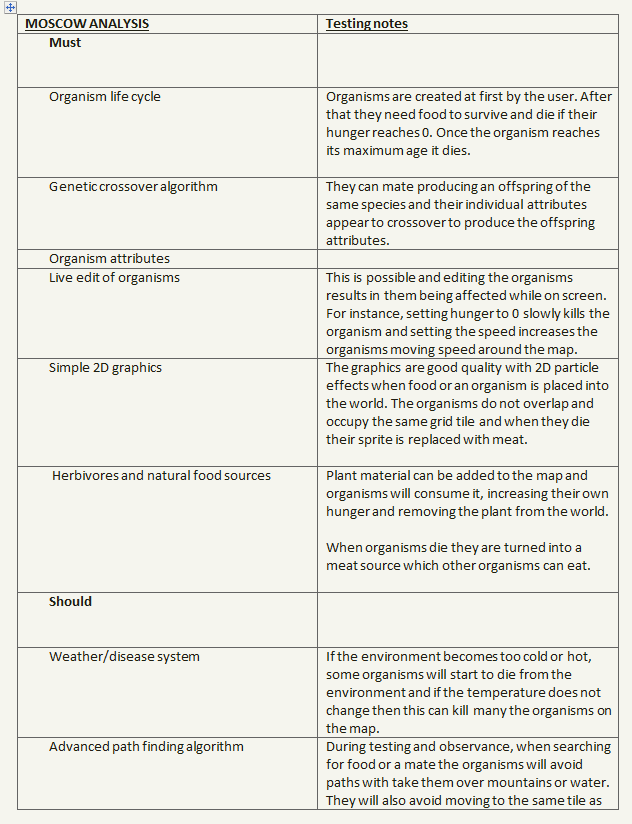
\includegraphics[width=1\textwidth]{testing-1}
\end{figure}

\begin{figure}[H]
	\caption{Requirements Testing}
	\centering
	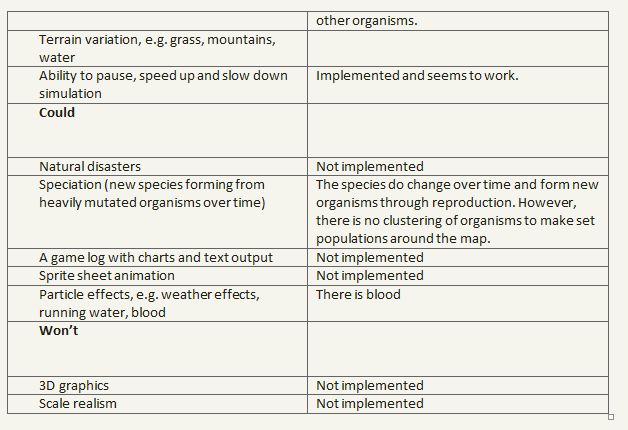
\includegraphics[width=1\textwidth]{testing-2}
\end{figure}

\end{document}

